\documentclass[10pt,french]{book}

\input preambule_2013
\pagestyle{empty}

\usepackage{geometry} % package offrant une autre méthode pour redéfinir les marges
\geometry{a4paper, top=1cm,bottom=1cm,left=1cm,right=1cm}

\newcommand\presentation{
\setcounter{exo}{0}
    \begin{tabular}{ll}
        Nom : \\[5pt]
        Prénom :
    \end{tabular}
\hfill
    \textbf{Note :}
        \renewcommand\arraystretch{2.3}
    \begin{tabular}{|c|}
        \hline
            \slashbox{\Huge\bfseries\phantom{10}}{\Huge\bfseries 10}\\
        \hline
    \end{tabular}
        \renewcommand\arraystretch{1.5}\par
    \vspace{1cm}
    \hrulefill
}


\begin{document}

\begin{landscape}
\presentation

\begin{multicols}{2}

\exo Dans le repère \OIJ ci-dessous, représenter les droites ci-dessous \textbf{en respectant les couleurs}. \textbf{Attention à bien détailler la démarche.}
\begin{enumerate}
    \item \textbf{En bleu} : $(d_1) : y = 2x - 1$.
    \item \textbf{En rouge} : $(d_2) : y = \dfrac{-1}{3} x + 2$.
    \item \textbf{En vert} : $(d_3) : x = 1,5$.
\end{enumerate}\medskip

\exo Dans chaque cas, déterminer l'équation de la droite à l'aide des coordonnées de deux points de la droite. \textbf{Ne pas dessiner les droites !}
\begin{enumerate}
    \item $(d_4)$ passant par $R(2 \pv 3)$ et $S(1 \pv 4)$.
    \item $(d_5)$ passant par $T(-1 \pv -2)$ et $U(2 \pv 0)$.
    \item $(d_6)$ passant par $V(4\pv 6)$ et $W(4 \pv -4)$.
\end{enumerate}

\begin{center}
    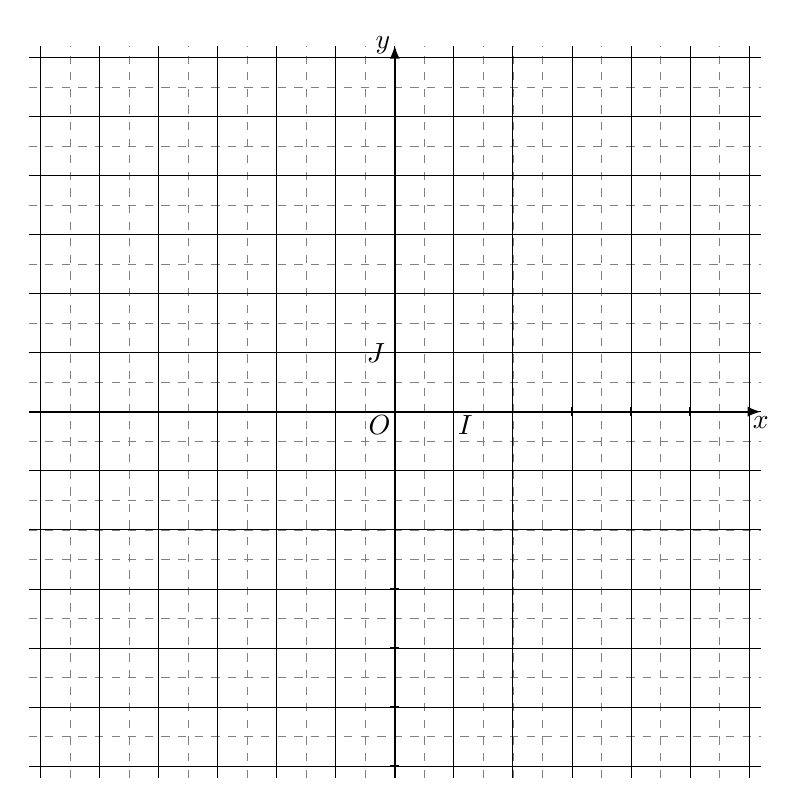
\begin{tikzpicture}[>=latex,scale=0.75]
        \def\xmin{-6.2} \def\xmax{6.2} \def\ymin{-6.2} \def\ymax{6.2}
        \draw[help lines, dashed] (\xmin,\ymin) grid[step=0.5cm] (\xmax,\ymax);
        \draw[line width = 0.25pt] (\xmin,\ymin) grid (\xmax,\ymax);
        \draw[->,line width = 0.65pt] (\xmin,0) -- (\xmax,0) node[below=-2pt] {$x$};
        \draw[->,line width = 0.65pt] (0,\ymin) -- (0,\ymax) node[left=-2pt] {$y$};
        \coordinate (O) at (0,0); \draw (O) node[below left = -2pt] {$O$};
        \coordinate (I) at (1,0); \draw (I) node[below right = -2pt] {$I$}; \foreach \x in {-6,...,6}  \draw (\x,-0.075)--(\x,0.075);
        \coordinate (J) at (0,1); \draw (J) node[left] {$J$}; \foreach \x in {-6,...,6} \draw (-0.075,\x)--(0.075,\x);
    \end{tikzpicture}
\end{center}

\columnbreak

\textbf{Calculs :}

\end{multicols}


\clearpage

%--------------------------------------------------------------------------------------------------------------------------------------------------------------------------
%                           SUJET B
%--------------------------------------------------------------------------------------------------------------------------------------------------------------------------

\presentation

\begin{multicols}{2}

\exo Dans le repère \OIJ ci-dessous, représenter les droites ci-dessous \textbf{en respectant les couleurs}. \textbf{Attention à bien détailler la démarche.}
\begin{enumerate}
    \item \textbf{En rouge} : $(d_1) : y = -2x + 1$.
    \item \textbf{En vert} : $(d_2) : y = \dfrac{1}{4} x - 2$.
    \item \textbf{En bleu} : $(d_3) : x = -2,5$.
\end{enumerate}\medskip

\exo Dans chaque cas, déterminer l'équation de la droite à l'aide des coordonnées de deux points de la droite. \textbf{Ne pas dessiner les droites !}
\begin{enumerate}
    \item $(d_4)$ passant par $R(1 \pv 3)$ et $S(2 \pv 4)$.
    \item $(d_5)$ passant par $T(-1 \pv 2)$ et $U(2 \pv 0)$.
    \item $(d_6)$ passant par $V(2\pv 6)$ et $W(2 \pv -4)$.
\end{enumerate}

\begin{center}
    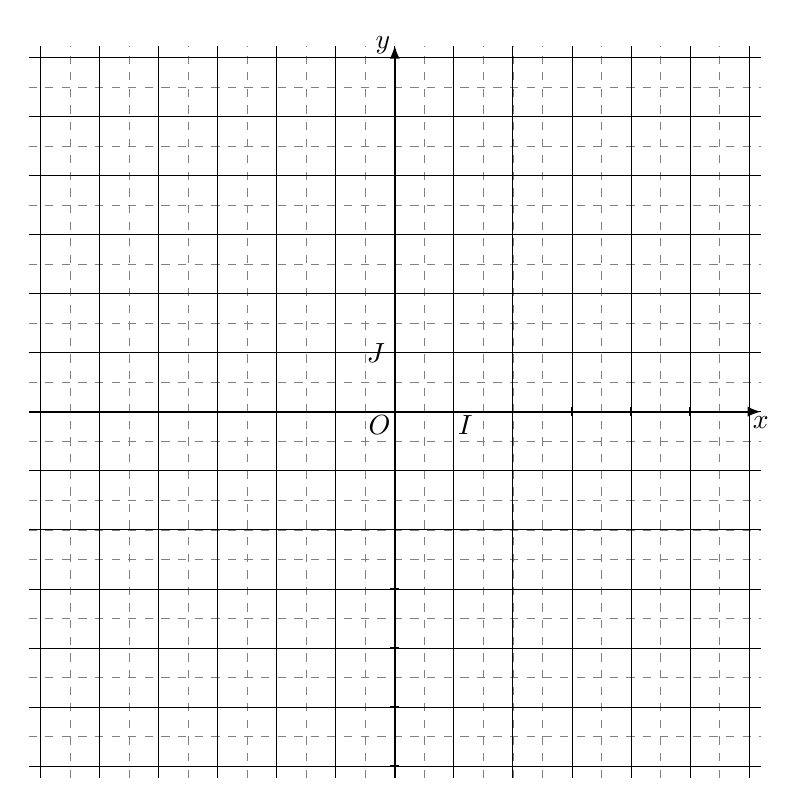
\begin{tikzpicture}[>=latex,scale=0.75]
        \def\xmin{-6.2} \def\xmax{6.2} \def\ymin{-6.2} \def\ymax{6.2}
        \draw[help lines, dashed] (\xmin,\ymin) grid[step=0.5cm] (\xmax,\ymax);
        \draw[line width = 0.25pt] (\xmin,\ymin) grid (\xmax,\ymax);
        \draw[->,line width = 0.65pt] (\xmin,0) -- (\xmax,0) node[below=-2pt] {$x$};
        \draw[->,line width = 0.65pt] (0,\ymin) -- (0,\ymax) node[left=-2pt] {$y$};
        \coordinate (O) at (0,0); \draw (O) node[below left = -2pt] {$O$};
        \coordinate (I) at (1,0); \draw (I) node[below right = -2pt] {$I$}; \foreach \x in {-6,...,6}  \draw (\x,-0.075)--(\x,0.075);
        \coordinate (J) at (0,1); \draw (J) node[left] {$J$}; \foreach \x in {-6,...,6} \draw (-0.075,\x)--(0.075,\x);
    \end{tikzpicture}
\end{center}

\columnbreak

\textbf{Calculs :}

\end{multicols}
\end{landscape}

\end{document} 